% ----- ----- ----- ----- ----- ----- ----- ----- ----- ----- ----- ----- ----- ----- -----
% Introductions
% ----- ----- ----- ----- ----- ----- ----- ----- ----- ----- ----- ----- ----- ----- -----

\clearpage

\onecolumn{
    \chapter{Introduction}

    \section{Abstract}

    This report covers the training and evaluation of Logistic Regression (LR), Random Forest (RF), and K Nearest Neighbors (KNN) machine learning models on a dataset for 
    \href{https://www.kaggle.com/datasets/kamilpytlak/personal-key-indicators-of-heart-disease}{Indicators Of Heart Disease}. The aforementioned dataset was taken from a survey of close to 400,000 individuals where
    the aim was to identify major risk factors associated with heart disease. The data that was collected to populate this dataset was collected from the United States including all 50 states, Washington D.C., and other
    U.S. territories. The aim of the models that were trained from this data set was to predict the presence of heart disease in an individual based upon the features used in the dataset.

    Once the tuned models were trained they were evaluated with a multitude of metrics. These metrics include Confusion matrices, ROC curves, and AUC scores. Upon evaluation of all three models the model that was found to perform
    the best was the Random Forest model.
}

\twocolumn


% ----- ----- ----- ----- ----- ----- ----- ----- ----- ----- ----- ----- ----- ----- -----
% Data Preparation And EDA
% ----- ----- ----- ----- ----- ----- ----- ----- ----- ----- ----- ----- ----- ----- -----

\clearpage

\chapter{Data Preparation And EDA}

\section{Data Preparation}

Upon downloading the data set from Kaggle, the data from the CSV was cleaned to make it digest-able for the future models. The dataset itself was comprised of the following features:

\begin{itemize}
    \item \textbf{BMI} - Body Mass Index, float.
    \item \textbf{Smoking} - Smoking status, categorical, casted to binary.
    \item \textbf{Alcohol} - Alcohol consumption, categorical, casted to binary.
    \item \textbf{Stroke} - Stroke status, categorical, casted to binary.
    \item \textbf{Physical Health} - Physical health status, float.
    \item \textbf{Mental Health} - Mental health status, float.
    \item \textbf{Difficulty Walking} - Difficulty walking status, categorical, casted to binary.
    \item \textbf{Sex} - Sex of person, casted to binary, 1 female, 0 males.
    \item \textbf{Age Category} - Age category of person, categorical:
    \begin{itemize}
        \item \textbf{18-24}: 0
        \item \textbf{25-29}: 1
        \item \textbf{30-34}: 2
        \item \textbf{35-39}: 3
        \item \textbf{40-44}: 4
        \item \textbf{45-49}: 5
        \item \textbf{50-54}: 6
        \item \textbf{55-59}: 7
        \item \textbf{60-64}: 8
        \item \textbf{65-69}: 9
        \item \textbf{70-74}: 10
        \item \textbf{75-79}: 11
        \item \textbf{80 Or Older}: 12
    \end{itemize}
    \item \textbf{Race} - Race of person, categorical:
    \begin{itemize}
        \item \textbf{American Indian/Alaskan Native}: 0
        \item \textbf{Asian}: 1
        \item \textbf{Black/African American}: 2
        \item \textbf{Hispanic/Latino}: 3
        \item \textbf{Other}: 4
        \item \textbf{White}: 5
    \end{itemize}
    \item \textbf{Diabetic} - Diabetic status, categorical, casted to binary.
    \item \textbf{Physical Activity} - Physical activity status, categorical, casted to binary.
    \item \textbf{Gen Health} - General health status, categorical:
    \begin{itemize}
        \item \textbf{Poor}: 0
        \item \textbf{Fair}: 1
        \item \textbf{Good}: 2
        \item \textbf{Very good}: 3
        \item \textbf{Excellent}: 4
    \end{itemize}
    \item \textbf{Sleep Time} - Sleep time, float.
    \item \textbf{Asthma} - Asthma status, categorical, casted to binary.
    \item \textbf{Kidney Disease} - Kidney disease status, categorical, casted to binary.
    \item \textbf{Skin Cancer} - Skin cancer status, categorical, casted to binary.
\end{itemize}

Overall, this dataset had a total of 17 features and 319,795 entries. Once the data was cleaned, it was then split into training and testing sets with a 80/20 split respectively.

% ----- ----- ----- ----- ----- ----- ----- ----- ----- ----- ----- ----- ----- ----- -----
% Model Selection And Tuning
% ----- ----- ----- ----- ----- ----- ----- ----- ----- ----- ----- ----- ----- ----- -----

\clearpage

\chapter{Model Selection And Tuning}

\section{Model Selection}

The three models that were used for training with dataset were:

\begin{itemize}
    \item \textbf{Logistic Regression} - Model was used in this context because it is a relatively simple model that can be used to predict binary outcomes.
    \item \textbf{Random Forest} - Similar to Logistic Regression, this model can be used to predict binary outcomes with more complexity.
    \item \textbf{K Nearest Neighbors} - Lastly, a KNN model was also used to predict binary outcomes thanks to its simplicity and ease of use.
\end{itemize}

For each of the models that were listed above, each had their own hyper tuning of the parameters. The purpose of this was a desire to find the best possible model for each individual model.

\subsec{Logistic Regression Fine Tuning}

The tuning of the Logistic Regression model was done with the use of \textbf{GridSearchCV} (Grid Search Cross Validation). The purpose of this was to determine the best combination of parameters that would produce
the best performance. The primary parameters that were tuned were penalty, C, and solver. The penalty parameter specifies the type of method used to prevent overfitting where as the C parameter controls the inverse of this method. The
solver parameter was used to specify the algorithm to use in the optimization problem.

Once all the combinations were evaluated, the optimal regression model was then selected based upon the highest cross-validation accuracy. The best hyperparamters were then passed off to retrain the model on the training data. The model
was then saved after being trained so it could later be used to evaluate the model.

\subsec{Random Forest Fine Tuning}

The tuning of the Random Forest model was done with the use of \textbf{RandomizedSearchCV} (Randomized Search Cross Validation) to efficiently explore a wide range of hyperparameters and identify the best 
combination for maximizing performance. The main parameters that were tuned included n\_estimators, max\_depth, min\_samples\_split, min\_samples\_leaf, and bootstrap. The n\_estimators parameter controls 
the number of trees in the forest, while max\_depth limits the depth of each individual tree to prevent overfitting. The min\_samples\_split and min\_samples\_leaf parameters specify the minimum number of 
samples required to split a node and form a leaf node, respectively, which helps in regulating the complexity of the model. The bootstrap parameter determines whether sampling with replacement is used when 
building the trees, which can impact the robustness of the model.

\textbf{RandomizedSearchCV} randomly sampled 50 different combinations of these parameters (n\_iter=50) and evaluated each using 3-fold cross-validation (cv=3). This approach was chosen because it is more 
computationally efficient than an exhaustive grid search, especially given the complexity of the Random Forest model. After evaluating all combinations, the best-performing hyperparameters were identified and 
used to retrain the model on the full training dataset. The optimized model was then saved so that it could later be used for testing and final evaluation on unseen data.

\subsec{K Nearest Neighbors Fine Tuning}

The tuning of the K-Nearest Neighbors (KNN) model was done using \textbf{GridSearchCV} (Grid Search Cross Validation) to find the best set of hyperparameters for optimal model performance. The main parameters 
that were tuned included n\_neighbors, weights, and metric. The n\_neighbors parameter specifies the number of neighbors considered during classification, which influences the smoothness of decision boundaries. 
The weights parameter determines whether each neighbor contributes equally (uniform) or is weighted by distance (distance). The metric parameter specifies the distance function used to calculate similarity 
between points, with options such as euclidean, manhattan, and minkowski.

The \textbf{GridSearchCV} method was used to evaluate all combinations of these parameters using 3-fold cross-validation (cv=3). This approach systematically tests each parameter setting, allowing for an 
exhaustive search of the defined hyperparameter space. After evaluating all the combinations, the best-performing hyperparameters were identified and used to retrain the KNN model on the full training dataset. 
The optimized KNN model was then saved for subsequent evaluation on the test data to assess its predictive performance on unseen samples.

% ----- ----- ----- ----- ----- ----- ----- ----- ----- ----- ----- ----- ----- ----- -----
% Model Evaluation
% ----- ----- ----- ----- ----- ----- ----- ----- ----- ----- ----- ----- ----- ----- -----

\clearpage

\chapter{Model Evaluation}

\subsec{Methodology}

The evaluation of these models included using the built in metrics from the \textbf{sklearn} library. The metrics that were used to evaluate the models included the following:

\begin{itemize}
    \item \textbf{classification\_report} - A built in report that shows the
    \begin{itemize}
        \item \textbf{Precision} - The ratio of correctly predicted positive observations to the total predicted positives.
        \item \textbf{Recall} - The ratio of correctly predicted positive observations to the all observations in actual class.
        \item \textbf{F1-Score} - The weighted average of Precision and Recall.
        \item \textbf{Support} - The number of actual occurrences of the class in the specified dataset.
    \end{itemize}
    of a model.
    \item \textbf{confusion\_matrix} - A matrix that shows the number of true positives, false positives, true negatives, and false negatives.
    \item \textbf{roc\_curve} - A curve that shows the true positive rate against the false positive rate.
\end{itemize}

These metrics were explicitly chosen because of the binary nature of the dataset that was used in this model. The classification report that is included in \textbf{sklearn} gives basic statistics about the model's
performance. The confusion matrix gives a visual representation of the types of decisions that were made against the test data set where we can see what it guessed versus what the true answer is. And lastly, the ROC curve
gives a visual representation of the overall performance of the model where we can see the true positive rate against the false positive rate. All of these metrics can give us an indication of how well the model is performing
as well as where it could possibly improve.

\subsec{General Statistics}

As mentioned previously, the built in classification report was used to evaluate the models in a purely quantitative manner. Since this  model is a binary classification model, each model that was trained had the aforementioned
statistics for both the positive and negative classes. The first model that was evaluated was the Logistic Regression model. The statistics for this model can be seen below.

\small{
    \begin{table}[h]
        \centering
        \begin{tabular}{|c|c|c|c|c|}
            \hline \textbf{Bin} & \textbf{Precision} & \textbf{Recall} & \textbf{F1-Score} & \textbf{Support} \\ \hline
            0 & 0.92 & 0.99 & 0.96 & 56,784 \\ \hline
            1 & 0.51 & 0.11 & 0.17 & 5,307 \\ \hline
        \end{tabular}
        \caption*{\textit{Classification Report for Logistic Regression Model}}
    \end{table}
}

A more thorough discussion of the results from the model as well as others as a whole will be discussed in the conclusion section, however, immediate observations from the results produced by the classification report show that the model is
performing well for the negative class, but not so well for the positive class. We can see this visually later on we observe the Confusion matrix and ROC curve.

The next model that was evaluated was the Random Forest model. The statistics for this model can be seen below.

\small{
    \begin{table}[h]
        \centering
        \begin{tabular}{|c|c|c|c|c|}
            \hline \textbf{Bin} & \textbf{Precision} & \textbf{Recall} & \textbf{F1-Score} & \textbf{Support} \\ \hline
            0 & 0.92 & 1.00 & 0.96 & 56,784 \\ \hline
            1 & 0.59 & 0.04 & 0.08 & 5,307 \\ \hline
        \end{tabular}
        \caption*{\textit{Classification Report for Random Forest Model}}
    \end{table}
}

Immediate observations show that the Random Forest model is performing slightly better when it comes to classifying the positive class. However, the model is still not performing well as a whole when it comes to the positive class. The negative class
is performing well however and the possible causes for this discrepancy with all models will be discussed later.

The last model that was evaluated was the K Nearest Neighbors model. The statistics for this model can be seen below.

\small{
    \begin{table}[h]
        \centering
        \begin{tabular}{|c|c|c|c|c|}
            \hline \textbf{Bin} & \textbf{Precision} & \textbf{Recall} & \textbf{F1-Score} & \textbf{Support} \\ \hline
            0 & 0.92 & 1.00 & 0.96 & 56,784 \\ \hline
            1 & 0.52 & 0.02 & 0.04 & 5,307 \\ \hline
        \end{tabular}
        \caption*{\textit{Classification Report for K Nearest Neighbors Model}}
    \end{table}
}

Similar performance when it comes to the positive class is observed for the K Nearest Neighbors model as it was for the Logistic Regression model. We now move on to the visual representation of the models performance.

\subsec{Confusion Matrices}

The intention of the confusion matrix is to give a visual representation of the models performance. The confusion matrix shows the number of true positives, false positives, true negatives, and false negatives. 
We can first visualize the confusion matrix for the Logistic Regression model.

\begin{figure}[h]
    \centering
    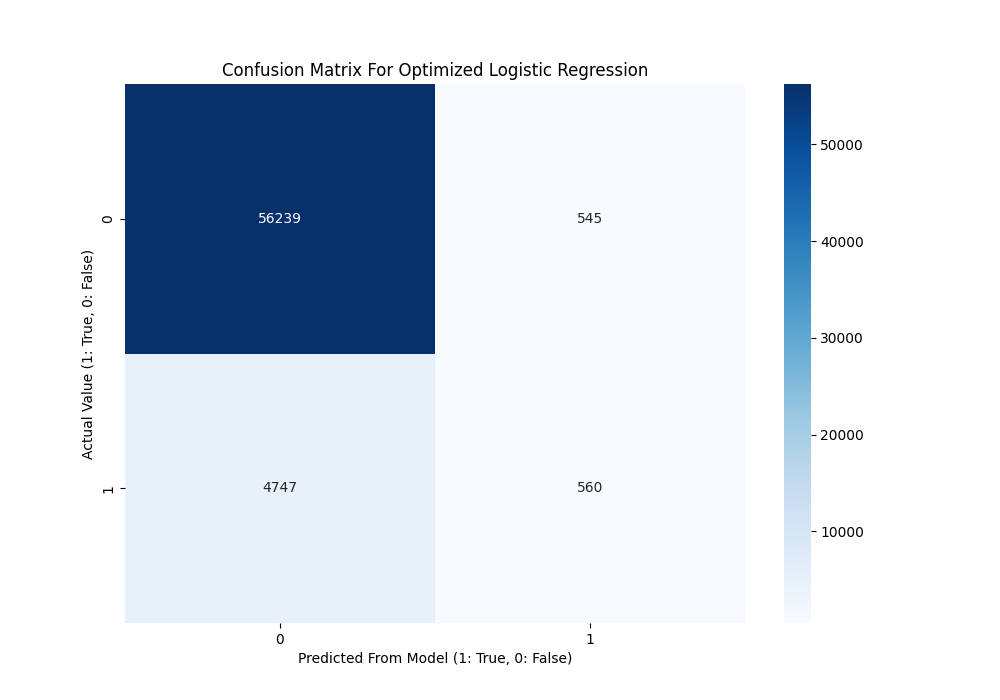
\includegraphics[width=0.5\textwidth]{"Images/LR CM.png"}
\end{figure}

From the above image we can see that the true negatives is the most common prediction that the model makes and also the most accurate. The false positives however is the least common prediction that model makes. Immediate observations
indicate that this model is performing well for the negative class, but not so well for the positive class.

Next, we can visualize the confusion matrix for the Random Forest model.

\begin{figure}[h]
    \centering
    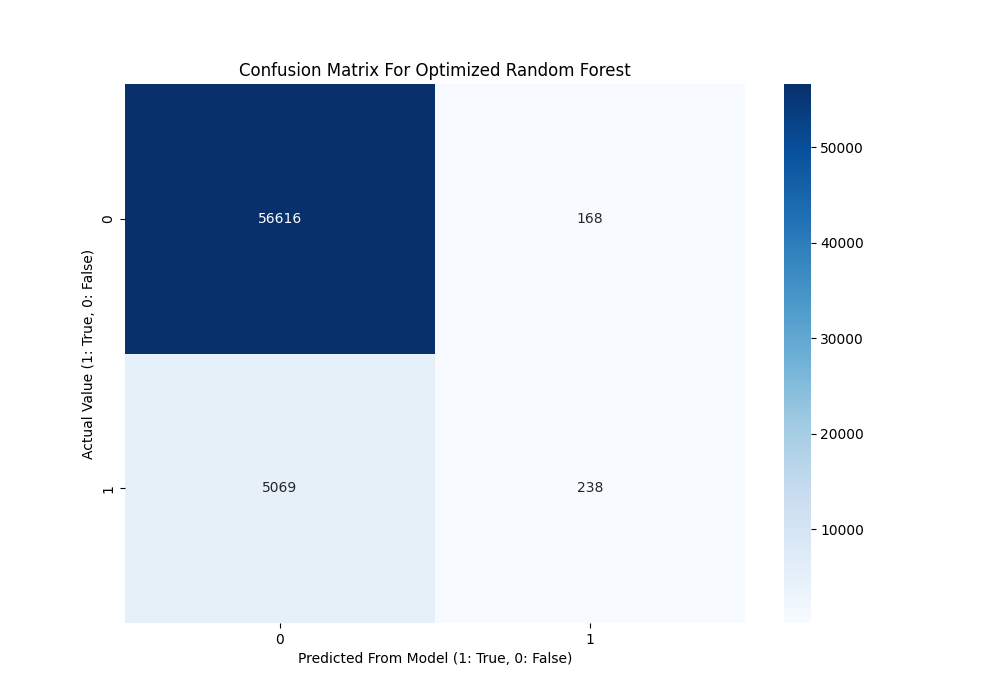
\includegraphics[width=0.5\textwidth]{"Images/RF CM.png"}
\end{figure}

Immediate comparisons to the Logistic Regression model show that there is slightly more true negative predictions for the Random Forest model as well as significantly less true positives. This indicates that the model is still not
performing well for the positive class.

Lastly, we can visualize the confusion matrix for the K Nearest Neighbors model.

\begin{figure}[h]
    \centering
    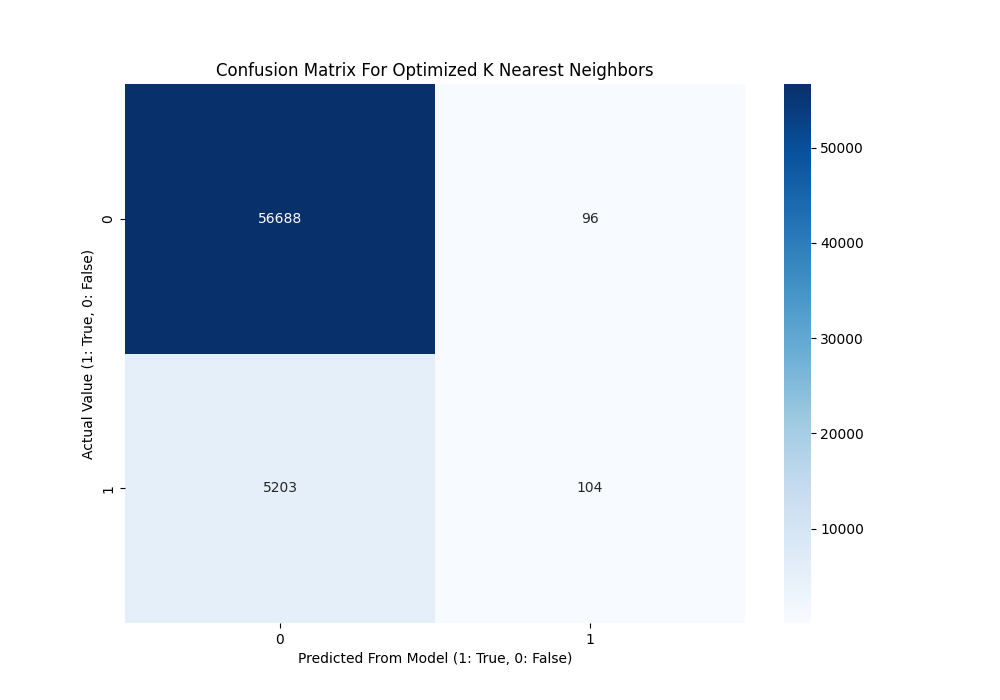
\includegraphics[width=0.5\textwidth]{"Images/KNN CM.png"}
\end{figure}

The trend that was observed in the Random Forest model with the true negatives increasing and the true positives decreasing is also observed in the K Nearest Neighbors model. In fact, the results for the positive class in the KNN model
diminished in comparison to the Random Forest model.

\subsec{ROC Curves}

The last metric that was used to evaluate the models was an ROC curve. The ROC curve shows the true positive rate against the false positive rate. With a binary classification model, one can interpret the ROC curve as a measure of the model's
ability to make correct predictions versus random guessing. We first observe the ROC curve for the Logistic Regression model. 

\newpage

\begin{figure}[h]
    \centering
    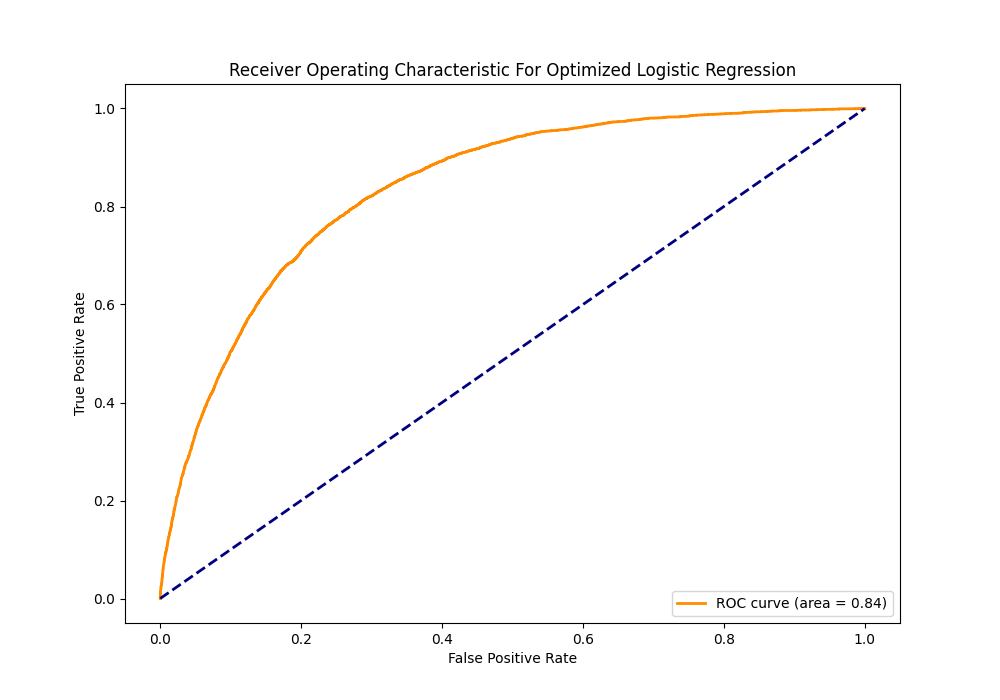
\includegraphics[width=0.45\textwidth]{"Images/LR ROC.png"}
\end{figure}

From the ROC curve that can be seen above, we can see that the model is already performing better than just random guessing. In the bottom right of the image, we can see that the area under the curve happens to be 0.84. This measure (the AUC)
is a statistical metric that describes the models ability to differentiate between positive and negative classes. The more up and to the left the ROC curve, the better. Since the AUC is 0.84, this would implicate that the Logistic
Regression model has a good ability of discriminating between classes for this dataset.

The next model that was evaluated was the Random Forest model.

\begin{figure}[h]
    \centering
    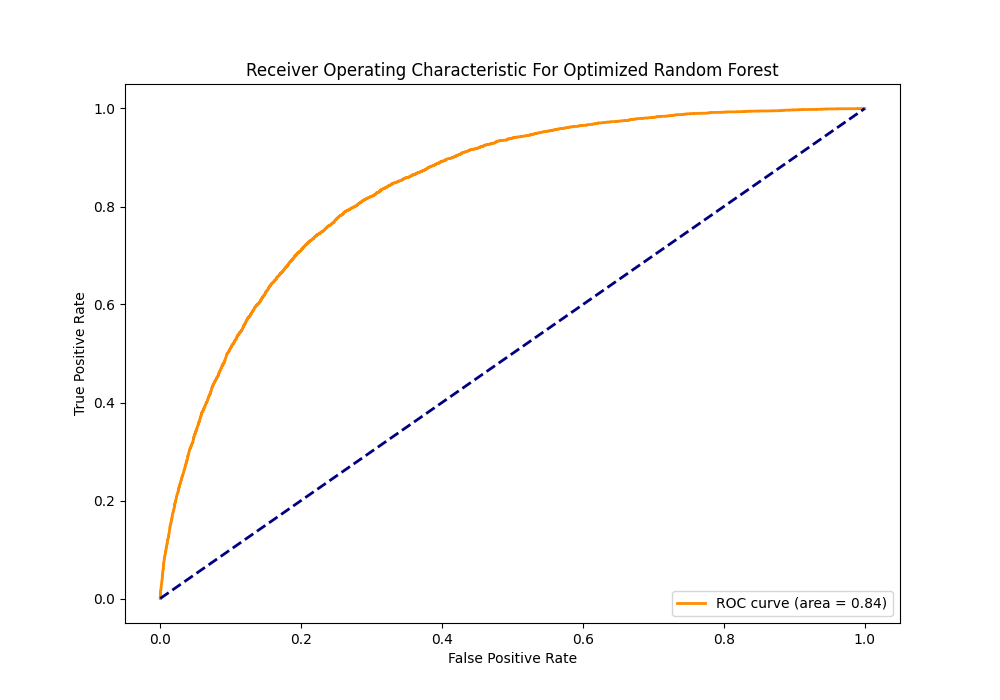
\includegraphics[width=0.45\textwidth]{"Images/RF ROC.png"}
\end{figure}

The results from the Random Forest confusion matrix are almost the exact same as the Logistic Regression model. The AUC for the Random Forest model is the same as that for the Logistic Regression model as well. From these results, we can
conclude that this model also has good discriminating ability.

The last model that was evaluated was the K Nearest Neighbors model.

\begin{figure}[h]
    \centering
    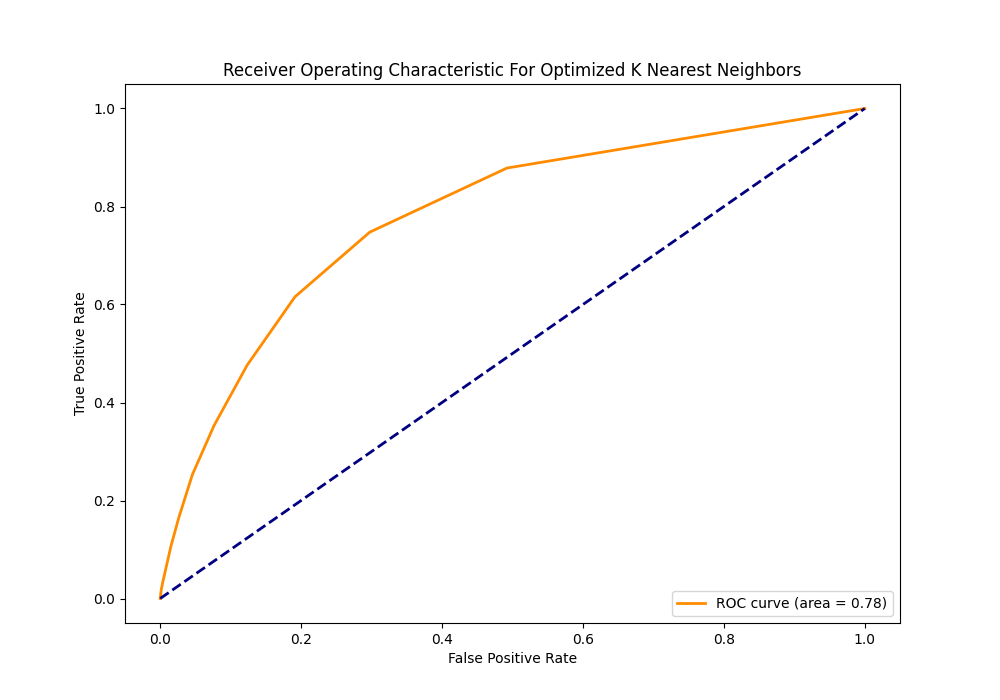
\includegraphics[width=0.45\textwidth]{"Images/KNN ROC.png"}
\end{figure}

The results from the K Nearest Neighbors model implicate that it is the worst performing model. The metric that is used to determine this is the AUC. With an AUC of 0.78, this model has the worst discriminating ability of the three models
that were trained on this dataset. It isn't performing necessarily poorly, but it is worse than the other two models.

% ----- ----- ----- ----- ----- ----- ----- ----- ----- ----- ----- ----- ----- ----- -----
% Conclusion
% ----- ----- ----- ----- ----- ----- ----- ----- ----- ----- ----- ----- ----- ----- -----

\clearpage

\chapter{Conclusion}

\section{Summary}

The dataset that was used in this project consisted of features that were collected in survey responses from individuals in the hopes of identifying major risk factors associated with heart disease. The dataset was comprised of 17 features
and had nearly 400,000 total entries. Three machine learning models were hypertuned so that the best possible subset of a model was chosen before being trained on this dataset. The Logistic Regression and Random Forest models had an AUC
score of 0.84 that was the highest amongst the Logistic Regression, Random Forest, and K Nearest Neighbors models implicating that the Logistic Regression and Random Forest models had the best discriminating ability.

Upon evaluation of all three models, it was discovered that the ability for the models to accurately predict true positive classes was very poor in comparison to the ability to detect true negative classes. Regardless of the hypertuning that
was done in the training of the model, each model struggled severely with accurately predicting if someone had heart disease. The cause for this can be outside of the control of what was done to train these models. When it comes to predicting
a biological condition such as a disease, it usually is a very complicated model to accurately create. One could increase the number of features in the model to see if that would increase the accuracy, but chances are that it would still be
very difficult to accurately predict true positive classes.

The causes as to why the Logistic Regression and Random Forest models performed better than that of the K Nearest Neighbors model could be due to the nature of the problem that this model is trying to solve. All models were trained to make
a binary classification. One could argue that the reason why the Logistic Regression model performs better in contrast to the the K Nearest Neighbors model is due to relationship between the features being linear. Conversely, if the relationship
were nonlinear between the features, then the Random Forest model would perform better than the K Nearest Neighbors model. This is because the Random Forest model is able to capture the nonlinearity of the data.

K Nearest Neighbor models usually are more sensitive to outliers in comparison to the other two models. This is a potential cause as to why it performed so poorly. Regardless of the model, the difficulty in accurately predicting whether or not
an individual has heart disease is a very difficult problem to solve regardless of the method being used. If one answered questions in a survey that aligned with the features in this dataset, and used one of these models to determine if they
were are risk for heart disease, if the model said you didn't have heart disease it would be correct far more times in comparison to when it wouldn't. The likelihood that the model would be correct if it told you that you were at risk for
heart disease would be very low.

% ----- ----- ----- ----- ----- ----- ----- ----- ----- ----- ----- ----- ----- ----- -----
% Appendix
% ----- ----- ----- ----- ----- ----- ----- ----- ----- ----- ----- ----- ----- ----- -----

\clearpage

\onecolumn{
    \chapter{Appendix}

    \section{Source Code}
    
    \begin{highlight}[Assets]
        The following is the code for the function that was used to prep the data from the csv.

    \begin{code}[Python]
    ''' PrepData - Prepares the data for training
            Input:
                data - The name of the data file
            Algorithm:
                * Read the data
                * Replace string values with numerical values
                * Drop rows with missing values in the 'HeartDisease' column
                * Save the cleaned data back to the CSV file
            Output:
                [X, Y] - The features and target values
    '''
    def PrepData(data):
        # Data Cleaning
        df = pd.read_csv(f'../Data/{data}.csv') # Read the data
        df = df.replace({"Yes": 1, "No": 0}) # Replace string values with numerical values
        df = df.replace({"Female": 1, "Male": 0}) # Replace string values with numerical values
        df = df.replace({
            "18-24": 0,
            "25-29": 1,
            "30-34": 2,
            "35-39": 3,
            "40-44": 4,
            "45-49": 5,
            "50-54": 6,
            "55-59": 7,
            "60-64": 8,
            "65-69": 9,
            "70-74": 10,
            "75-79": 11,
            "80 or older": 12,
        })
        df = df.replace({
            "American Indian/Alaskan Native": 0,
            "Asian": 1,
            "Black": 2,
            "Hispanic": 3,
            "Other": 4,
            "White": 5,
        }) # Replace string values with numerical values
        df = df[df['Diabetic'].isin([0,1])] # Drop rows with missing values in the 'Diabetic' column
        df = df.replace({
            "Poor": 0,
            "Fair": 1,
            "Good": 2,
            "Very good": 3,
            "Excellent": 4,
        }) # Replace string values with numerical values
        # Drop rows with missing values in the 'HeartDisease' column
        df = df.dropna(subset=['HeartDisease'])
        # Save the cleaned data back to the CSV file
        df.to_csv('../Data/Heart_Data.csv', index=False)
        X = df.drop('HeartDisease', axis=1)
        Y = df['HeartDisease']
        return [X, Y]
    \end{code}

        The following is the code for the function that was used to train a model.

    \begin{code}[Python]
    ''' TrainModel - Trains a model and saves it to a file
            Input:
                model - The model to train
                modelName - The name of the model
                x_train - The features of the training data
                y_train - The target values of the training data
                x_test - The features of the test data
            Algorithm:
                * Fit the model
                * Make predictions
                * Delete previous model if it exists
                * Save the model
            Output:
                [model, modelPred] - The trained model and its predictions
    '''
    def TrainModel(model, modelName, x_train, y_train, x_test):
        # Fit the model
        model.fit(x_train, y_train)
        # Make predictions
        modelPred = model.predict(x_test)
        # Delete previous model if it exists
        model_path = f"../Models/{modelName}.pkl"
        if os.path.exists(model_path):
            os.remove(model_path)
        # Save the model
        joblib.dump(model, model_path)
        return [model, modelPred]
    \end{code}

        The following is the code for the function that was used to evaluate a model.

    \begin{code}[Python]
    ''' AnalyzeModel - Analyzes a model that was previously trained
            Input:
                modelName - The name of the model to analyze
                x_test - The features of the test data
                y_test - The target values of the test data
            Algorithm:
                * Load the model
                * Make predictions
                * Print the classification report
                * Create a confusion matrix and display it
                * Create an ROC curve and display it if the model supports probability predictions
            Output:
                None
    '''
    def AnalyzeModel(modelName, x_test, y_test):
        # Load the model
        model = joblib.load(f"../Models/{modelName}.pkl")
        # Make predictions
        predictions = model.predict(x_test)
        # Print the classification report
        print(f"Model - {modelName}, Classification Report:")
        print(classification_report(y_test, predictions))
        # Create Confusion Matrix
        cm = confusion_matrix(y_test, predictions)
        plt.figure(figsize=(10, 7))
        sns.heatmap(cm, annot=True, fmt="d", cmap='Blues')
        plt.xlabel('Predicted From Model (1: True, 0: False)')
        plt.ylabel('Actual Value (1: True, 0: False)')
        plt.title(f"Confusion Matrix For {modelName}")
        plt.show()
        # Create ROC Curve if model supports probability predictions
        if hasattr(model, "predict_proba"):
            probs = model.predict_proba(x_test)[:, 1]
            fpr, tpr, thresholds = roc_curve(y_test, probs)
            roc_auc = auc(fpr, tpr)
            plt.figure(figsize=(10, 7))
            plt.plot(fpr, tpr, color='darkorange', lw=2, label='ROC curve (area = %0.2f)' % roc_auc)
            plt.plot([0, 1], [0, 1], color='navy', lw=2, linestyle='--')
            plt.xlabel('False Positive Rate')
            plt.ylabel('True Positive Rate')
            plt.title(f'Receiver Operating Characteristic For {modelName}')
            plt.legend(loc="lower right")
            plt.show()
        else:
            print(f"{modelName} does not support probability predictions.")        
    \end{code}

        Lastly, the function that was used to run the program.
        
    \begin{code}[Python]
    ''' Run - Runs the program
            Input:
                None
            Algorithm:
                * Prepare the data
                * Split the data into training and testing sets
                * Train and analyze the models
            Output:
                None
    '''
    def Run():
        # Data
        X, Y = PrepData("Heart_Data")
        x_train, x_test, y_train, y_test = train_test_split(X, Y, test_size=0.2, random_state=42)
        def LR():
            ## Logistic Regression - Hyperparameter Tuning
            logReg = LogisticRegression(max_iter=2000)
            param_grid_logReg = {
                'penalty': ['l2'],  # 'l1', 'elasticnet' could be considered if 'liblinear' or 'saga' solver is used
                'C': [0.001, 0.01, 0.1, 1, 10, 100],  # Regularization strength
                'solver': ['lbfgs', 'liblinear', 'saga'],
            }
            grid_search_logReg = GridSearchCV(logReg, param_grid_logReg, cv=3, n_jobs=-1, verbose=2)
            logReg_opt = grid_search_logReg.fit(x_train, y_train)
            logReg_best = logReg_opt.best_estimator_

            # Train and Analyze the Best Logistic Regression Model
            logReg_best, logRegPred = TrainModel(logReg_best, "Optimized Logistic Regression", x_train, y_train, x_test)
            print("Logistic Regression Model Trained")
            return [logReg_best, logRegPred]
        def RF():
            # ## Random Forest - Hyperparameter Tuning
            rf = RandomForestClassifier(random_state=42)
            param_grid_rf = {
                'n_estimators': [100, 200, 300],               # Number of trees in the forest
                'max_depth': [10, 20, 30, None],               # Depth of the tree
                'min_samples_split': [2, 5, 10],               # Minimum samples required to split an internal node
                'min_samples_leaf': [1, 2, 4],                 # Minimum samples required to be at a leaf node
                'bootstrap': [True, False]                     # Whether bootstrap samples are used when building trees
            }
            random_search_rf = RandomizedSearchCV(rf, param_distributions=param_grid_rf, n_iter=50, cv=3, random_state=42, n_jobs=-1, verbose=2)
            rf_opt = random_search_rf.fit(x_train, y_train)
            rf_best = rf_opt.best_estimator_

            # Train and Analyze the Best Random Forest Model
            rf_best, rfPred = TrainModel(rf_best, "Optimized Random Forest", x_train, y_train, x_test)
            print("Random Forest Model Trained")
            return [rf_best, rfPred]
        def KNN():
            ## K Nearest Neighbors - Hyperparameter Tuning
            knn = KNeighborsClassifier()
            param_grid_knn = {
                'n_neighbors': [3, 5, 7, 9, 11, 15, 20],       # Number of neighbors to use
                'weights': ['uniform', 'distance'],            # Weight function used in prediction
                'metric': ['euclidean', 'manhattan', 'minkowski']  # Distance metric for neighbors
            }
            grid_search_knn = GridSearchCV(knn, param_grid_knn, cv=3, n_jobs=-1, verbose=2)
            knn_opt = grid_search_knn.fit(x_train, y_train)
            knn_best = knn_opt.best_estimator_

            # Train and Analyze the Best KNN Model
            knn_best, knnPred = TrainModel(knn_best, "Optimized K Nearest Neighbors", x_train, y_train, x_test)
            print("K Nearest Neighbors Model Trained")
            return [knn_best, knnPred]
        # Choices
        inp = input("Train Models (1), Evaluate Models (2), or Exit (3)? ")
        # Train Models
        if inp == "1":
            inputTrain = input("Train Logistic Regression (1), Random Forest (2), K Nearest Neighbors (3), or All (4)? ")
            # Logistic Regression
            if inputTrain == "1":
                LR()
            # Random Forest
            elif inputTrain == "2":
                RF()
            # K Nearest Neighbors
            elif inputTrain == "3":
                KNN()
            # All
            elif inputTrain == "4":
                LR()
                RF()
                KNN()
            return
        # Evaluate
        elif inp == "2":
            inputEval = input("Evaluate Logistic Regression (1), Random Forest (2), K Nearest Neighbors (3), or All (4)? ")
            # Logistic Regression
            if inputEval == "1":
                AnalyzeModel("Optimized Logistic Regression", x_test, y_test)
            # Random Forest
            elif inputEval == "2":
                AnalyzeModel("Optimized Random Forest", x_test, y_test)
            # K Nearest Neighbors
            elif inputEval == "3":
                AnalyzeModel("Optimized K Nearest Neighbors", x_test, y_test)
            # All
            elif inputEval == "4":
                AnalyzeModel("Optimized Logistic Regression", x_test, y_test)
                AnalyzeModel("Optimized Random Forest", x_test, y_test)
                AnalyzeModel("Optimized K Nearest Neighbors", x_test, y_test)
        # Other
        elif inp == "3":
            return
        return
    \end{code}
    \end{highlight}

    \begin{highlight}[Main]
        Below is the code for the main file that was used to run the program.

    \begin{code}[Python]
    from assets import *

    if __name__ == "__main__":
        Run()
    \end{code}

        And the modules / libraries that were used in this project.

    \begin{code}[Python]
    from sklearn.model_selection import train_test_split
    from sklearn.linear_model import LogisticRegression
    from sklearn.ensemble import RandomForestClassifier
    from sklearn.neighbors import KNeighborsClassifier
    from sklearn.metrics import classification_report, confusion_matrix, roc_curve, auc
    from sklearn.model_selection import GridSearchCV, RandomizedSearchCV
    import joblib
    import pandas as pd
    import seaborn as sns
    import os
    import matplotlib.pyplot as plt
    \end{code}
    \end{highlight}
}

% ----- ----- ----- ----- ----- ----- ----- ----- ----- ----- ----- ----- ----- ----- -----
% Resources
% ----- ----- ----- ----- ----- ----- ----- ----- ----- ----- ----- ----- ----- ----- -----

\clearpage

\chapter{Resources}

\section{Sources}

\begin{itemize}
    \item \textbf{Confusion Matrix} - \href{https://en.wikipedia.org/wiki/Confusion_matrix}{Confusion Matrix}, source explaining the confusion matrix.
    \item \textbf{Dataset} - \href{https://www.kaggle.com/datasets/kamilpytlak/personal-key-indicators-of-heart-disease}{Kaggle Dataset}, dataset used for this project.
    \item \textbf{joblib} - \href{https://joblib.readthedocs.io/en/stable/}{Documentation}, library used to save the trained models.
    \item \textbf{matplotlib} - \href{https://matplotlib.org/stable/contents.html}{Documentation}, library used to create visualizations.
    \item \textbf{pandas} - \href{https://pandas.pydata.org/docs/}{Documentation}, library used to read and manipulate the data.
    \item \textbf{ROC Curve} - \href{https://en.wikipedia.org/wiki/Receiver_operating_characteristic}{ROC Curve}, source explaining the ROC curve.
    \item \textbf{scikitlearn} - \href{https://scikit-learn.org/0.21/documentation.html}{Documentation}, library used to train and evaluate the models.
    \item \textbf{seaborn} - \href{https://seaborn.pydata.org/}{Documentation}, library used to create visualizations.
\end{itemize}